\newpage
\section{Cache}

\subsection{Introduction}

A significant characteristic of the hardware development during the last decades has been the increasing \textbf{gap} between \textbf{processor cycle time} and \textbf{main memory access time}. 
\underline{Example 1 (Memory latency)}: let's consider a processor operating at 1 GHz (1 ns clock) connected to a DRAM with a latency of 100 ns, and if we assume that processor has two ALU units and it is capable of executing two instructions in each cycle of 1 ns, then the peak processor rating is 2 GFLOPS (Giga Float.Pt. Ops per Sec). However, since the memory latency is equal to 100 cycles every time a memory request is made, the processor must wait 100 cycles before it can process the data.

To use processor cycles efficiently, a \textbf{memory hierarchy} is typically used, consisting of multiple levels of memories with different sizes and access times. Only the main memory on the top of the hierarchy is built from DRAM, the other levels use \textbf{SRAM} (static random access memory), and the resulting memories are often called \textbf{caches}. The goal in the design of a memory hierarchy is to be able to access a \textbf{large percentage of the data from a fast memory}, and only a small fraction of the data from the slow main memory, thus leading to a small average memory access time. The simplest form of a memory hierarchy is the use of a single cache between the processor and main memory (one-level cache, L1 cache), but nowadays two or three levels of cache are used for each processor. Note that for multiprocessor systems, there exists an additional problem, the so-called \textbf{cache coherence problem}, i.e. it must be ensured that a processor accessing a data element always accesses the most recently written value.

In general, the access times of caches are 0.5-2.5 ns, while for the DRAM are 50-70 ns. We can consider a cache system as the following:

\begin{figure}[h!]
		\centering
		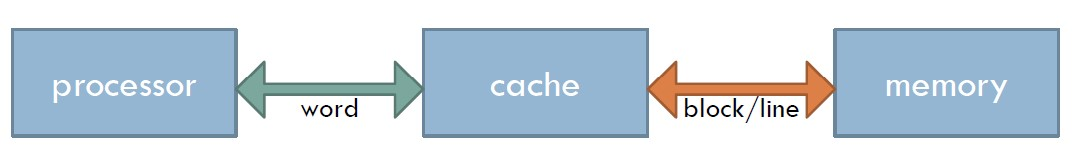
\includegraphics[scale = 1.2]{img/cache.jpg}
        \label{cache}
        \caption{Cache system}
\end{figure}

\begin{itemize}

    \item the data needed by the processor is first fetched into the cache (cache hit or miss), then all subsequent accesses to data items residing in the cache are serviced by the cache. The \textbf{cache hit ratio} is defined as the fraction of memory references that are resolved by the cache memory;
    
    \item performance improves in presence of \textit{high locality}:

    \begin{itemize}
    
        \item \textit{temporal locality}: a data item is re-used after a short amount of time;

        \item \textit{spatial locality}: data with close memory addresses is used within a short amount of time.
        
    \end{itemize}

    \item data transport between cache and main memory is done by the transfer of blocks comprising several words, whereas the processor accesses single words in the cache.
    
    
\end{itemize}

\underline{Example 2 (Memory latency with cache)}: let's consider a processor operating at 1 GHz (1 ns clock) connected to a DRAM with a latency of 100 ns and suppose that we have a cache of 32KB, with a latency of 1 ns per word, and we consider the problem of multiplying two matrices $A$ and $B$ of size 32*32 (we suppose that $A$, $B$ and $A * B$ fit in the cache). Then, the time needed to load $A$ and $B$ into the cache is $32*32*2* 100 ns = 205 \mu s$. Then, multiplying two matrices of size n*n takes $2n^3$ multiply-adds, in our case $2*32^3 = 66K$ multiply-adds, which implies $66 \mu s$. Finally, the total time is $205 + 66 = 271 \mu s$, so the throughput is $\frac{66K * 2}{271} = 488$ MFLOPS (> $10$ MFLOPS of the Example 1) (still < $2$ GFLOPS, which represents the peak processor rating). Moreover, we underline the fact that the locality is exploited by observing that the computational complexity of these operations is $n^3$, but here we are computing using $n^2$ memory locations!


\underline{Example 3 (Bandwidth with cache)}: let's consider the previous example. If the \textit{cache block} has a width of \textit{one single word}, then it takes $32*32*2*100 ns = 205 \mu s$ to load the two matrices in cache. However, if the width is of \textit{four words}, then the overhead is $32*32*2/4*100 ns = 51 \mu s$, with a total time (load into cache + computation) of $51 + 66 = 117 \mu s$. In this case, the throughput is $\frac{66K * 2}{117} = 1282$ MFLOPS (> 488 MFLOPS of Example 2) (> 10 MFLOPS of Example 1) (still < 2 GFLOPS of the peak processor rating).

Along with cache coherence problem, another important issue for the cache is the \textbf{cache-to-memory coherence}, i.e. the problem consisting on when to write to the memory data that have been modified in the cache. There exist two possible alternatives:

\begin{itemize}

    \item \textbf{write-through policy}, i.e. data is immediately written to memory, so a downside is that the write operation is delayed, while the pro is that the memory is always consistent with the content of the cache;

    \item \textbf{write-back policy}, i.e. memory is updated upon eviction. In this case the two major downsides are that the content of the memory may differ from the content of the cache (inconsistency) and that the processor may not need anymore the data that is currently in the cache. An example of inconsistency is represented in the following picture: the processors see different values of $u$ after the event 3.

    \begin{figure}[h!]
		\centering
		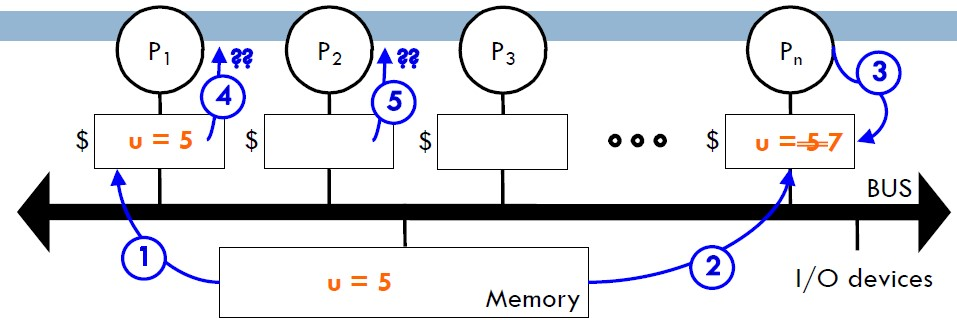
\includegraphics[scale = 0.8]{img/inconsistency.jpg}
        \label{inconsistency}
        \caption{Inconsistency problem}
    \end{figure}
    
    On the other hand, this policy results in having less writing operations;

    \item \textbf{snooping protocols}, most of which assumes that local caches of the processors use a write-through policy and that all memory accesses are performed via the central bus. In this way, each cache controller can observe all write accesses to perform updates or invalidations
    
\end{itemize}

Finally, one last example of important issue concerning cache is the \textbf{false sharing}, which happens when two \textit{unrelated variables}, i.e. variables that are logically private to distinct threads, are allocated in the same block and do not conflict. In this case, from the point of view of the data block the accesses are considered conflicts, even if the two processors access disjoint words of the same block, thus the cache updates are not necessary! In this sense, it is usually a good practice to put on the same block \textit{related variables}.

\subsection{Models}
So far we've seen that the cache has a significant impact on the performance of modern applications, so now we focus both on the cache models and on some algorithms that exploit the cache use, in particular \textit{matrix multiplication} and \textit{sorting}.

\subsubsection{External-Memory Model}
Before analyzing the \textit{cache-oblivious model}, we first review the standard model of a two-level memory hierarchy with block transfers. This model is known as \textbf{external-memory model}, and it defines the computer as having two levels, as represented in Picture \ref{external_memory_model}:

\begin{itemize}
    \item the \textit{cache} which is near to the CPU, cheap to access but limited in space;
    \item the \textit{disk} which is distant from the CPU, expensive to access but nearly limitless in space.
\end{itemize}


\begin{figure}[h!]
		\centering
		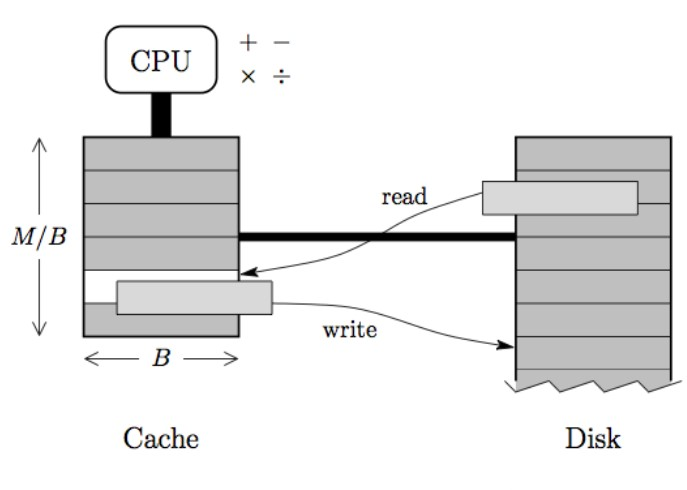
\includegraphics[scale = 1.2]{img/model.jpg}
        \label{external_memory_model}
        \caption{External-Memory model}
\end{figure}

The central aspect of this model is that transfers between \textit{cache} and \textit{disk} involve \textit{blocks} of data: as we can see, each block has size $B$, while the \textit{cache} has size $M \geq B^2$ and contains $M/B$ entries. The main properties of this model are:

\begin{itemize}

    \item it provides a simple description of the relationship between CPU, \textit{cache} and \textit{disk};

    \item the complexity of the algorithms we will consider will be based on the number of \textit{disk} accesses;

    \item the algorithms will be optimized for specific values of $M$ and $B$;

    \item we assume that the cache is working in the best possible way, i.e. it always makes the best possible choices.
    
\end{itemize}

\subsubsection{Cache-Oblivious Model}
The other important cache model is the \textbf{cache-oblivious model}, and its basic idea is to design external-memory algorithms without knowing $B$ and $M$. But this simple idea has several surprisingly powerful \textbf{consequences}:

\begin{itemize}
    \item If a cache-oblivious algorithm performs well between two levels of the memory hierarchy (nominally called \textit{cache} and \textit{disk}), then it must automatically work well between any two adjacent levels of the memory hierarchy;
    \item If the number of memory transfers is optimal up to a constant factor between any two adjacent memory levels, then any weighted combination of these counts (with weights corresponding to the relative speeds of the memory levels) is also within a constant factor of optimal;
    \item The cache-oblivious model does not require to tune the cache parameters, an operation which make the code portability difficult: using this model, an algorithm should work well on all machines without modification.
\end{itemize}

In contrast to the external-memory model, algorithms in the cache-oblivious models \textbf{cannot explicitly manage the cache}, and this is necessary since both $M$ and $B$ are not known. Moreover, this model is based on several \textbf{assumptions}:

\begin{enumerate}
    \item the \textit{ideal cache model} assumes that the \textit{page replacement} operation is \textit{optimal}: in particular, it specifies that the page replacement strategy knows the future and always evicts the page that will be accessed farthest in the future. Real-world caches do not know the future, and employ more realistic page replacement strategies such as evicting the least-recently-used block (\textit{LRU}) or evicting the oldest block (\textit{FIFO});
    \item \textit{Full associativity}, i.e. we assume that any block can be stored anywhere in the cache, in contrast with real-world caches that are characterized by \textit{limited associativity};
    \item \textit{Tall-cache assumption}: the cache is assumed to be tall, i.e. $M = \Omega(B^2)$ (usually a weaker condition is sufficient $M = \Omega(B^{1 + \gamma})$, for any constant $\gamma > 0$). This property is particularly important in some of the more sophisticated cache-oblivious algorithms and data structures, where it ensures that the cache provides a polynomially large “buffer” for guessing the block size slightly wrong. It is also commonly assumed in external-memory algorithms.
\end{enumerate}

While on the one hand these assumptions are really strong, the following theorems make the model described above more feasible to be applied in order to deal with real-world problems, with the running time that degrades only by a constant factor:

\begin{itemize}
    \item \textbf{Lemma 1}: if an algorithm makes $T$ memory transfers on a cache of size $M/2$ with optimal replacement, then it makes at most $2T$ memory transfers on a cache of size $M$ with LRU or FIFO replacement. This means that LRU and FIFO replacement do just as well as optimal replacement up to a constant factor of memory transfers and up a constant factor wastage of the cache;
    \item \textbf{Lemma 2}: for some constant $\alpha > 0$, an LRU cache of size $\alpha M$ and block size $B$ can be simulated in $M$ space such that an access to a block takes $O(1)$ expected time. This result can be reached by using 2-universal has functions and by knowing both $B$ and $M$.
\end{itemize}

By this two theorems we cal conclude that a cache-oblivious model can be translated into a FIFO/LRU cache with 1-associativity paying only constant factors.

\subsection{Algorithms}
We now analyze some important techniques for designing \textbf{cache-oblivious algorithms}.

\subsubsection{Scanning}
The first problem we address is the problem of \textit{scanning}, in which our goal is to traverse all the elements of a set. On a flat memory hierarchy (uniform-cost RAM), such a procedure requires $\Theta(N)$ time for $N$ elements. In the external-memory model, if we store the elements in $\lceil N/B \rceil$ blocks of size $B$, then the number of blocks transfers is $\lceil N/B \rceil$.

To achieve a similar bound in the cache-oblivious model, we can lay out the elements of the set in a contiguous segment of memory, in any order, and implement the $N$-element traversal by scanning the elements one-by-one in the order they are stored: this layout and traversal algorithm do not require knowledge of $B$ (or $M$), and it is represented in Picture \ref{scanning}.

\begin{figure}[h!]
		\centering
		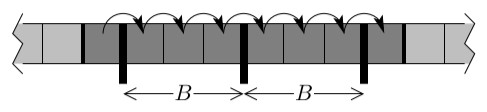
\includegraphics[scale = 1.2]{img/scanning.jpg}
        \label{scanning}
        \caption{Scanning problem in cache-oblivious model}
\end{figure}

The overall complexity using the cache-oblivious model is then $O(\lceil N/B \rceil) + 1$: as we can see, the cache-oblivious bound is an additive 1 away from the external-memory bound, and this is ideal, because normally our goal is to match bounds within multiplicative constant factors.

\subsubsection{Divide and Conquer}
After scanning, the first major technique for designing cache-oblivious algorithms is \textit{divide and conquer}, which often leads to algorithms whose memory-transfers count is optimal within a constant factor. 

The basic idea of this approach is that it \textbf{repeatedly refines the problem size}, until it will eventually \textbf{fit in the cache} (i.e. the size of the problem will be at most $M$) and, later, in a \textbf{single block} (i.e. the size will be at most $B$). The most important \textbf{property} of this approach is that if the number of leaves in the recursion tree is polynomially larger than the divide/merge cost, then the corresponding algorithm will use a number of memory transfers which is optimal within a constant factor.

We will now focus on a specific example of this approach, the \textit{matrix multiplication} problem.

\textbf{Matrix multiplication} \\
The problem of matrix multiplication consists of computing $C = A \cdot B$, where $A$ and $B$ being $N*N$ matrices. The first issue when considering this problem relies on how to store the matrices, and the two possibilities are (Picture \ref{row_column_major}):

\begin{itemize}

    \item \textit{row-major order}:in this case the elements of the matrix are stored by rows, so it is the preferable organization to store matrix $A$;

    \item \textit{column-major order}: in this case the elements of the matrix are stores by columns, so it is preferable organization to store matrix $B$.
    
\end{itemize}

\begin{figure}[h!]
		\centering
		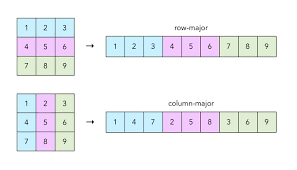
\includegraphics[scale = 0.9]{img/row_column_major.png}
        \label{row_column_major}
        \caption{Row-major order and column-major order representation}
\end{figure}

We can now take into considerations some algorithms to solve this problem.

\colorbox{yellow}{\underline{Algorithm 1}} (naive): this is the simplest algorithm, in which each element $C_{ij}$ is computed by scanning the $i$-th row of $A$ and the $j$-th column of $B$, where $A$ is stored in row-major order and $B$ is stored in column-major order. In this case, the \textbf{number of memory transfers} is given by:

$$
O(N^3/B + N^2)
$$

, since each element of $C$ involves a linear scanning of the row of $A$ and the column of $B$, i.e. $O(N/B + 1)$, and there are $N^2$ elements in $C$. A possible approach to reduce the cost of this algorithm consists of storing the row $i$ of $A$ in cache memory (if $M > N$), or to keep the matrix $A$ in cache (if $M > N^2$).

\colorbox{yellow}{\underline{Algorithm 2}} (external-memory model): this algorithms is based on the idea of multiplying the sub-matrices of $A$, $B$ and $C$, and the \textbf{optimal number of transfers} is $O(N^2/B + N^3/(B * \sqrt{M}))$

An important issue about this algorithm is the choice of the block size, and the optimal choice is to choose a block size $s$ such that $3*s^2 = M$, i.e. such that the cache can contain a block from $A$ and $B$, and that can store the result block of $C$.  

\colorbox{yellow}{\underline{Algorithm 3}} (cache oblivious): this algorithm exploits the \textit{divide-and-conquer} approach by recursively dividing the original matrix into sub-matrices until they fit into the cache, as represented in Picture \ref{mm_cache_oblivious}.

\begin{figure}[h!]
		\centering
		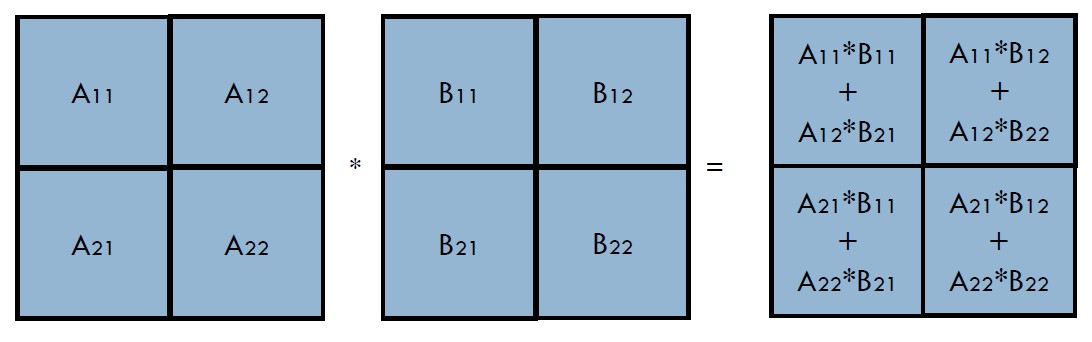
\includegraphics[scale = 0.9]{img/iimproved_algo.jpg}
        \label{mm_cache_oblivious}
        \caption{Divide-and-conquer approach for the matrix multiplication problem}
\end{figure}

Since we do not know in advance when a sub-matrix will fit into the cache, we need a recursive data layout such that however we recursively split the matrix, at some point all the data will be in (almost) consecutive memory locations that can be easily loaded in cache. An example of this organization is the \textit{Z-order representation}. 


The overall \textbf{number of transfers} of this algorithm is given by:

$$
O(N^2/B + N^3/(B \sqrt{M}))
$$

, so it has the same complexity of the external-memory model case.

This particular number of transfers is computed by solving the following recurrence:

$$
T(n) = 8T(N/2) + O(1 + N^2/B)
$$

, where:

\begin{itemize}
    \item $8T(N/2)$ represents the number of transfers of each of the eight multiplication subproblems;
    \item $O(1 + N^2/B)$ represents the number of transfers for each of the four addition subproblems
\end{itemize}


\subsubsection{Sorting} 
We now focus on the sorting problem.

\colorbox{yellow}{\underline{Merge-Sort}} (external-memory model): this algorithm works by recursively splitting the input vector into smaller sub-vectors (\textit{split phase}), by sorting them and by merging them together into the result sorted vector (\textit{merge phase}). We can easily notice that the main operation of the algorithm is represented by the merging phase. 

The best way of implementing this algorithm using an external-memory model is by using the $(M/B)$-way mergesort. In this case, during the merge each memory block maintains the first $B$ elements of each list, and when a block empties, the next block from that list is loaded. It can be shown this algorithm results in the following number of block transfers:

$$
\Theta(N/B \log_{M/B}(N/B))
$$

This number is computed by taking into account these informations:

\begin{itemize}
    \item the recursion tree has $\Theta(N/B)$ leaves;
    \item the leaf cost is $\Theta(N/B)$;
    \item the number of levels in the recursion tree is $\log_{M/B}N$
\end{itemize}

\colorbox{yellow}{\underline{Merge-Sort}} (cache oblivious): the goal of this algorithm is to run the merge phase, the most expensive one, in cache, for any value of $M$ and $B$. In particular, the provided solution consists of implementing a 2-way mergesort, whose complexity is:

$$
\Theta(N/B \log_2(N/M))
$$

Our next goal is then to find a method in order to improve this naive algorithm, in particular by rising the base of the logarithm in order to reach $M/B$. We will reach this goal by using the \textbf{k-funnel} and the \textbf{funnel-sort algorithm}.

\colorbox{yellow}{\underline{Funnelsort}} (cache oblivious): the core of this algorithm is characterized by the \textbf{k-funnel}, which is represented in Picture \ref{funnel}.

\begin{figure}[h!]
		\centering
		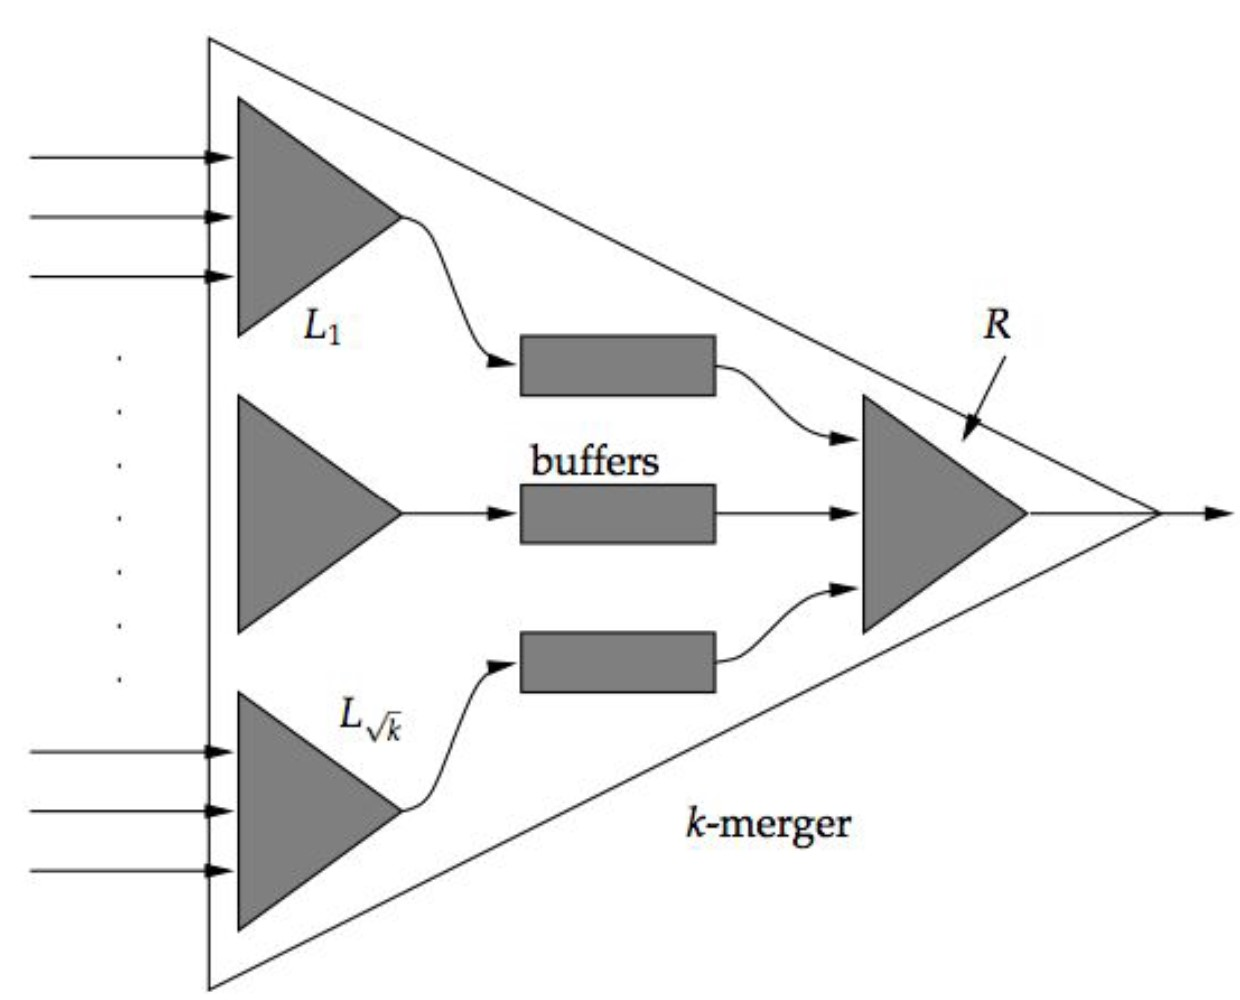
\includegraphics[scale = 0.5]{img/funnel.jpg}
        \label{funnel}
        \caption{k-funnel}
\end{figure}

A \textit{k-funnel} is a merger that merges $k$ sorted lists with total size $k^3 = N$ in a space $k^2$ (note that the cache locality is given by the $k^2 < k^3$ mismatch). More specifically, the \textit{k-funnel} receives in input $k$ sorted lists, that are partitioned into $\sqrt{k}$ groups of size $\sqrt{k}$: each group feeds a $\sqrt{k}$-funnel $L_i$. The output of each $L_i$ is stored in a buffer (FIFO) of size $2k^{3/2} = 2\sqrt{N}$: finally, the $\sqrt{k}$ buffers feed the $\sqrt{k}$-funnel $R$ whose output is the output of the \textit{k-funnel}. An important property of this merger is that if $R$ has buffer $i$ with less than $k^{3/2}$, it recursively invoke $L_i$.

The sizes of the \textit{k-funnel} are the following:

\begin{itemize}
    \item the size of each $L_i$ is $\sqrt{k} * \sqrt{k} = k$;
    \item $R$ has size $k$ as well;
    \item buffers has size $2 * k^{3/2}$
\end{itemize}

, so the total size of the merger is given by $(\sqrt{k} + 1)$ (number of funnels + $R$) + $\sqrt{k} * 2 * k^{3/2}$, which leads to $\Theta(k^2)$.
The \textit{funnelsort} algorithm is the first application of the tall-cache assumption: for simplicity, we assume that $M = \Omega(B^2)$, but the same result can be obtained when $M = \Omega(B^{1 + \gamma})$. Clearly, the crucial issue of this algorithm relies on the choice of the value of $k$: the larger the $k$, the faster the algorithm; however, $k$-funnel is fast only if it is fed at least $K^3$ elements. Thus, $k = N^{1/3}$ is chosen. The algorithm proceeds as follows:

\begin{enumerate}
    \item Split the array into $k = N^{1/3}$ contiguous segments, each of size $N/k = N^{2/3}$;
    \item Recursively sort each segment;
    \item Apply the $k$-funnel to merge the sorted segments.
\end{enumerate}

It can be proven that the \textbf{number of transfers} using the funnelsort algorithm is:

$$
\O(N/B \log_{M/B}(N/B))
$$

, i.e. it is the same as the mergesort using the external-memory model.

\underline{Example}: suppose that $N = 4,096 = 2^{12}$, then the operations of the funnelsort algorithm are:

\begin{enumerate}
    \item Split the array into $k = N^{1/3} = 2^4 = 16$ blocks, each of size $N/k = 2^8 = 256$;
    \item Sort each block independently;
    \item Merge the blocks with a $2^4 = 16$-funnel.
\end{enumerate}

Picture \ref{funnel1} represents the structure of the funnels, while Picture \ref{funnel2} shows the size of each component: note that each buffer has size $2 * k^{3/2} = 2 * 2^6 = 2^7 = 128$, and we recall that if $R$ has buffer $i$ with less than $k^{3/2} = 64$, it recursively invoke $L_i$.

\begin{figure}[h!]
		\centering
		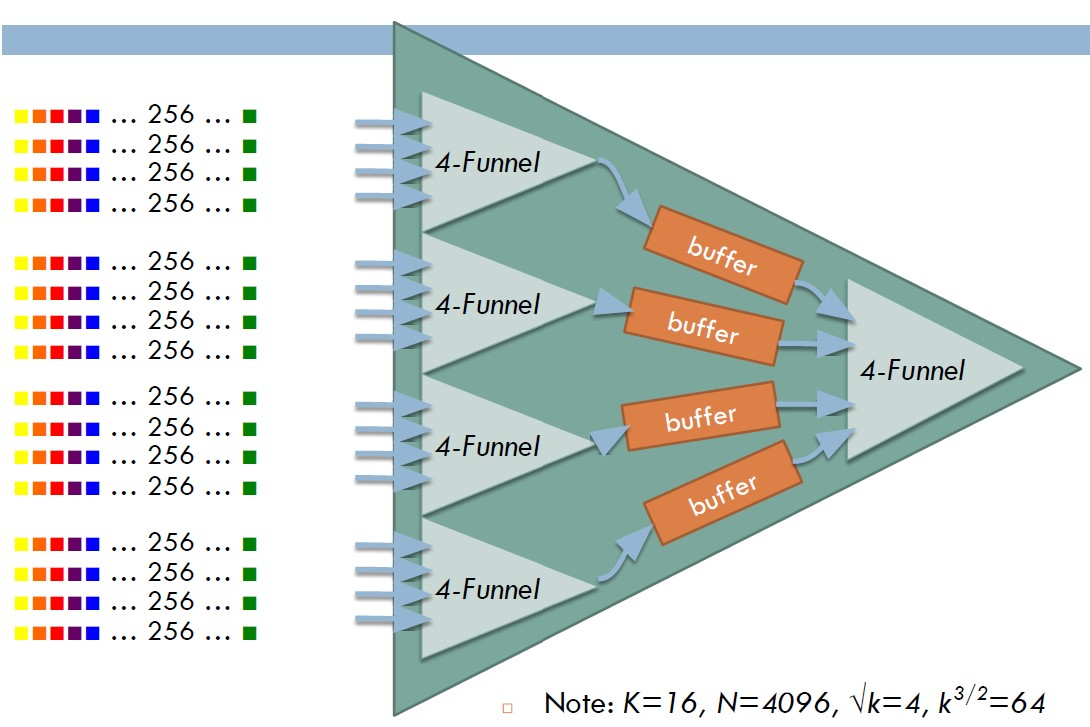
\includegraphics[scale = 0.7]{img/example_funnelsort_1.jpg}
        \label{funnel1}
        \caption{Example of 16-funnel: each buffer has size 128, while R has the same size of the funnel, i.e. 16}
\end{figure}

\begin{figure}[h!]
		\centering
		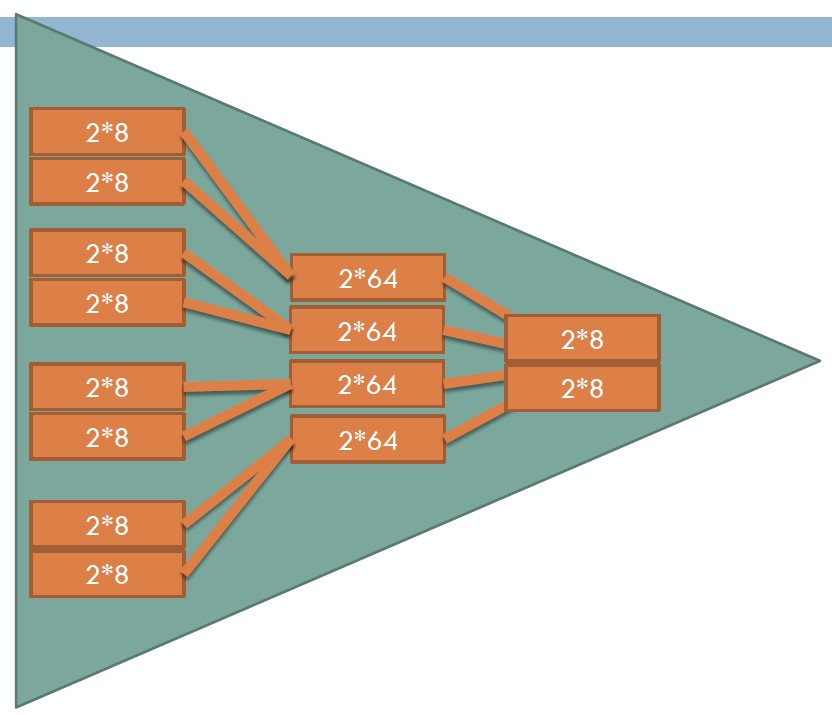
\includegraphics[scale = 0.7]{img/example_funnelsort_2.jpg}
        \label{funnel2}
        \caption{Sizes of the 16-funnel}
\end{figure}

Finally, another important issue about funnelsort is how to efficiently store a k-funnel. One possible solution could be to use a recursive layout, as represented in Picture \ref{funnel_recursive}.

\begin{figure}[h!]
		\centering
		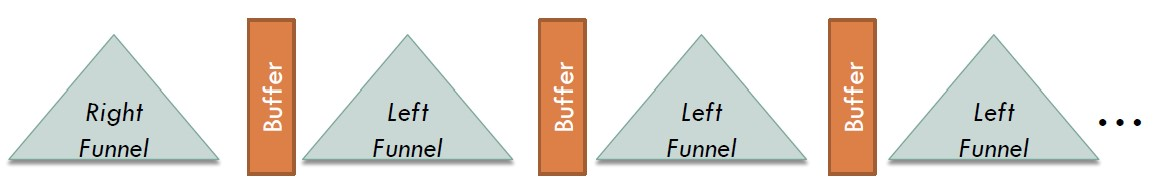
\includegraphics[scale = 0.8]{img/recursive_layout_funnels.jpg}
        \label{funnel_recursive}
        \caption{Recursive layout for a k-funnel}
\end{figure}

However, another possible approach could be to use the so called \textbf{lazy k-funnel}, which is represented as a binary tree of buffers (Picture \ref{lazy_kfunnel}), characterized by the following sizes:

\begin{figure}[h!]
		\centering
		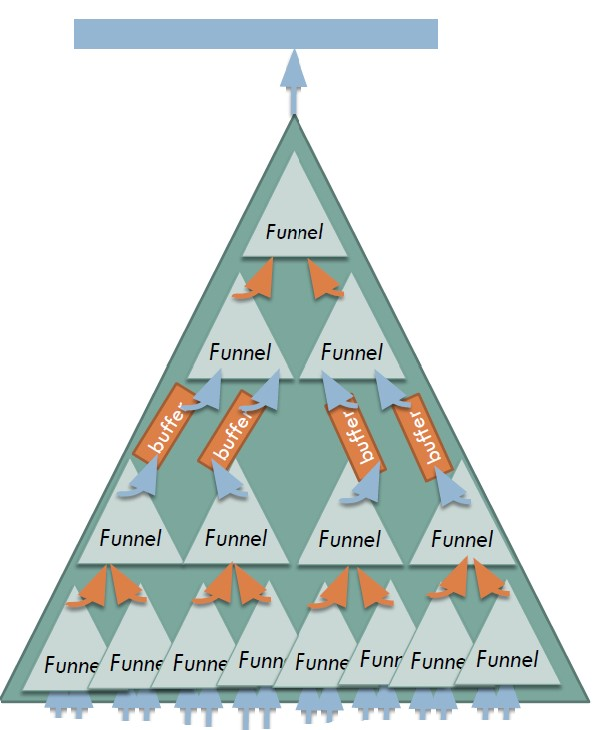
\includegraphics[scale = 0.8]{img/lazy_k_funnel.jpg}
        \label{lazy_kfunnel}
        \caption{Lazy k-funnel}
\end{figure}

\begin{itemize}
    \item the middle layer contains $2 ^ {\lceil \log(k)/2 \rceil}$ buffers, i.e. about $\sqrt{k}$ (in the picture, $k = 16$, so 4 buffers);
    \item each buffer has size $\lceil k^{3/2} \rceil$ (in the picture, the size is 64);
    \item the final buffer, containing the sorted elements, has size $k^3 = N$ (in the picture, $N = 2^{12}$).
\end{itemize}

One peculiarity of this lazy k-funnel is the FILL procedure, through which the buffers are filled, and it is defined as:

\begin{enumerate}
    \item While the buffer is not full:
    \begin{enumerate}
        \item If the left child is empty, then fill it;
        \item If the right child is empty, then fill it;
        \item Perform one merge step
    \end{enumerate}
\end{enumerate}

\subsection{Multicore Hierarchies: Key Challenge}
A crucial issue about the theory underlying the ideal cache model is that it falls apart once we introduce \textbf{parallelism}, i.e. good performances for any $M$ ans $B$ on a 2-level hierarchy do not imply good performances at all levels of hierarchy. This is mainly due to the fact that the \textbf{caches are not fully shared}, and for this reason the \textbf{scheduling} of \textbf{parallel threads} has a \textbf{large impact} on cache \textbf{performances}. Finally, the best technique to deal with caches and threads is to share a largely overlapping working set. 

\subsection{Other approaches}
Among other approaches for hiding the memory latency we can distinguish:

\begin{itemize}

    \item \textbf{multi-threading}, which consists in splitting the problem into multiple sub-problems and in running an independent thread for each sub-problem. Note that when a thread is idle on a miss, another thread can execute computational tasks;

    \item \textbf{pre-fetching}, which consists in anticipating load operations, so that data is already available when needed;

    \item \textbf{drawbacks}, which impact both on bandwidth and on cache pollution.
    
\end{itemize}
